% https://es.overleaf.com/latex/templates/project-report/jpzczmpsdzwm

%%% Preamble
\documentclass[paper=leter, fontsize=11pt]{scrartcl}
\usepackage[utf8]{inputenc}
\usepackage[spanish,mexico]{babel}
\usepackage[T1]{fontenc}    % use 8-bit T1 fonts
\usepackage{lmodern}
\usepackage{hyperref}       % hyperlinks
\usepackage{lipsum}
\usepackage[square,numbers]{natbib}

\usepackage[protrusion=true,expansion=true]{microtype}	
\usepackage{amsmath,amsfonts,amsthm} % Math packages
\usepackage[pdftex]{graphicx}
\usepackage{url}
 
\usepackage{booktabs}
\usepackage[table,xcdraw]{xcolor}

\usepackage{tikz}
\usetikzlibrary{positioning,matrix, arrows.meta}

\usepackage{caption} 
\usepackage{subcaption}


\usepackage{listings}
\lstdefinestyle{mystyle}{ 
    basicstyle=\ttfamily\footnotesize,
    breakatwhitespace=false,         
    breaklines=true,                 
    captionpos=b,                    
    keepspaces=true,                 
    numbers=left,                    
    numbersep=5pt,                  
    showspaces=false,                
    showstringspaces=false,
    showtabs=false,                  
    tabsize=4
}

\lstset{style=mystyle}
\renewcommand{\lstlistingname}{Código}


\selectlanguage{spanish}
\usepackage[spanish,onelanguage,ruled]{algorithm2e}


%%% Custom sectioning
\usepackage{sectsty}
\allsectionsfont{\centering \normalfont\scshape}


%%% Custom headers/footers (fancyhdr package)
\usepackage{fancyhdr}
\pagestyle{fancyplain}
\fancyhead{}											% No page header
\fancyfoot[L]{}											% Empty 
\fancyfoot[C]{}											% Empty
\fancyfoot[R]{\thepage}									% Pagenumbering
\renewcommand{\headrulewidth}{0pt}			% Remove header underlines
\renewcommand{\footrulewidth}{0pt}				% Remove footer underlines
\setlength{\headheight}{13.6pt}


%%% Equation and float numbering
\numberwithin{equation}{section}		% Equationnumbering: section.eq#
\numberwithin{figure}{section}			% Figurenumbering: section.fig#
\numberwithin{table}{section}				% Tablenumbering: section.tab#


%%% Maketitle metadata
\newcommand{\horrule}[1]{\rule{\linewidth}{#1}} 	% Horizontal rule

%%% https://tex.stackexchange.com/a/118217
\usepackage{mathtools}
\DeclarePairedDelimiter\ceil{\lceil}{\rceil}
\DeclarePairedDelimiter\floor{\lfloor}{\rfloor}

\usepackage{amsmath}

\usepackage{tikz}

\title{
		%\vspace{-1in} 	
		\usefont{OT1}{bch}{b}{n}
		\normalfont \normalsize \textsc{Posgrado de Ingeniería de Sistemas} \\ [25pt]
		\horrule{0.5pt} \\[0.4cm]
		\huge Transformaciones de datos \\
		\horrule{2pt} \\[0.5cm]
}
\author{
		\normalfont 								\normalsize
        Alberto Benavides\\[-3pt]		\normalsize
        \today
}
\date{}


%%% Begin document
\begin{document}
\maketitle

\section{Introducción}
En esta práctica se ha desarrollado una metodología computacional que permite comparar las correlaciones de ciertas funciones después de transformar sus variables de entrada y salida mediante las transformadas de Tuckey y de Box--Cox.

\section{Transformadas}

Las \emph{transformadas de Tuckey} \citep*{tuckey} parten de la idea de transformar variables independientes $X$ o dependientes $Y = f(X)$ en potencias de dichas variables $X^\lambda, Y^\lambda$ a partir de los distintos valores que pueda tomar $\lambda$, tal que
\begin{equation}
    z_\lambda = \left \{
        \begin{array}{ll}
        x^\lambda, & \text{ si } \lambda > 0, \\
                    \log (x), & \text{ si } \lambda = 0, \\
                    -(x^\lambda), & \text{ si } \lambda < 0.
        \end{array}
        \right .
\end{equation}

Por otro lado, las \emph{transformadas de Box--Cox} \citep*{boxcox}, por su cuenta, se realizan a partir de la ecuación
\begin{equation}
    z_\lambda = \frac{x^\lambda - 1}{\lambda}.
\end{equation}

\section{Correlaciones}

Ambas transformadas suelen usarse para mejorar la correlación de las funciones resultantes con respecto a la función original. Para ello, es posible transformar sólo $X$, $Y$ o ambas al mismo tiempo y luego calcular las correlaciones entre dichas variables. Así, una manera de encontrar la mejor transformada para una determinada función sería definir algunos valores de $\lambda$, transformarla mediante ambas transformadas y graficar las correlaciones de las funciones con transformaciones en $X$, $Y$ o ambas variables.

\section{Diseño de experimentos}
Se realiza un diseño de experimentos para comparar las correlaciones de las funciones transformadas a partir de las transformaciones de Tuckey y Box--Cox. Como ejemplo, se utilizan las funciones
\begin{itemize}
    \item $1 / x$,
    \item $x ^ 2$,
    \item $x ^ 3$,
    \item $\log (x)$,
    \item $e ^ x$,
    \item $\sin(x \cdot \frac{180}{\pi})$,
    \item $\cos(x \cdot \frac{180}{\pi})$,
    \item $\tan(x \cdot \frac{180}{\pi})$.
\end{itemize}

La variable  $\lambda = [-3.0, -2.5, -2.0, \ldots, 2.0, 2.5, 3.0 ]$, mientras que las transformaciones se aplican sobre sólo $X$, sólo $Y$ y ambas simultáneamente. Se generan mil valores de $X$ a partir de una distribución uniforme $\mathcal{U}(-100, 100)$ y se calculan $Y$ para cada función. Luego, se grafican las funciones de las transformadas de Tuckey y Box--Cox para cada una de estas variantes. Por último, se grafican las correlaciones con los distintos $\lambda$ tanto para las transformaciones de Tuckey como las de Box--Cox.

\section{Resultados}
Se muestran algunos ejemplos de esta práctica. Primero $1/x$. La función se muestra en la figura \ref{xTfunc3} (p. \pageref{xTfunc3}). El despliegue de correlaciones para las transformaciones de $X$, $Y$ y ambas se muestra en la figura \ref{corr3} (p. \pageref{corr3}). En dicha figura se puede apreciar que los valores de las correlaciones para ambas transformadas con los mismos valores $\lambda$ son iguales. Además, una animación de las diferentes transformaciones a lo largo de los cambios en $\lambda$ puede consultarse en \url{https://tinyurl.com/yxjepzdf}, \url{https://tinyurl.com/y468ba9o} y \url{https://tinyurl.com/y2e6a6w2} para las transformaciones de $X$, $Y$ y ambas, respectivamente. El resto de las funciones, comparaciones entre correlaciones, animaciones y el código se hallan en \url{https://github.com/jbenavidesv87/probabilidad/tree/master/tema7}.

\begin{figure}
    \centering
    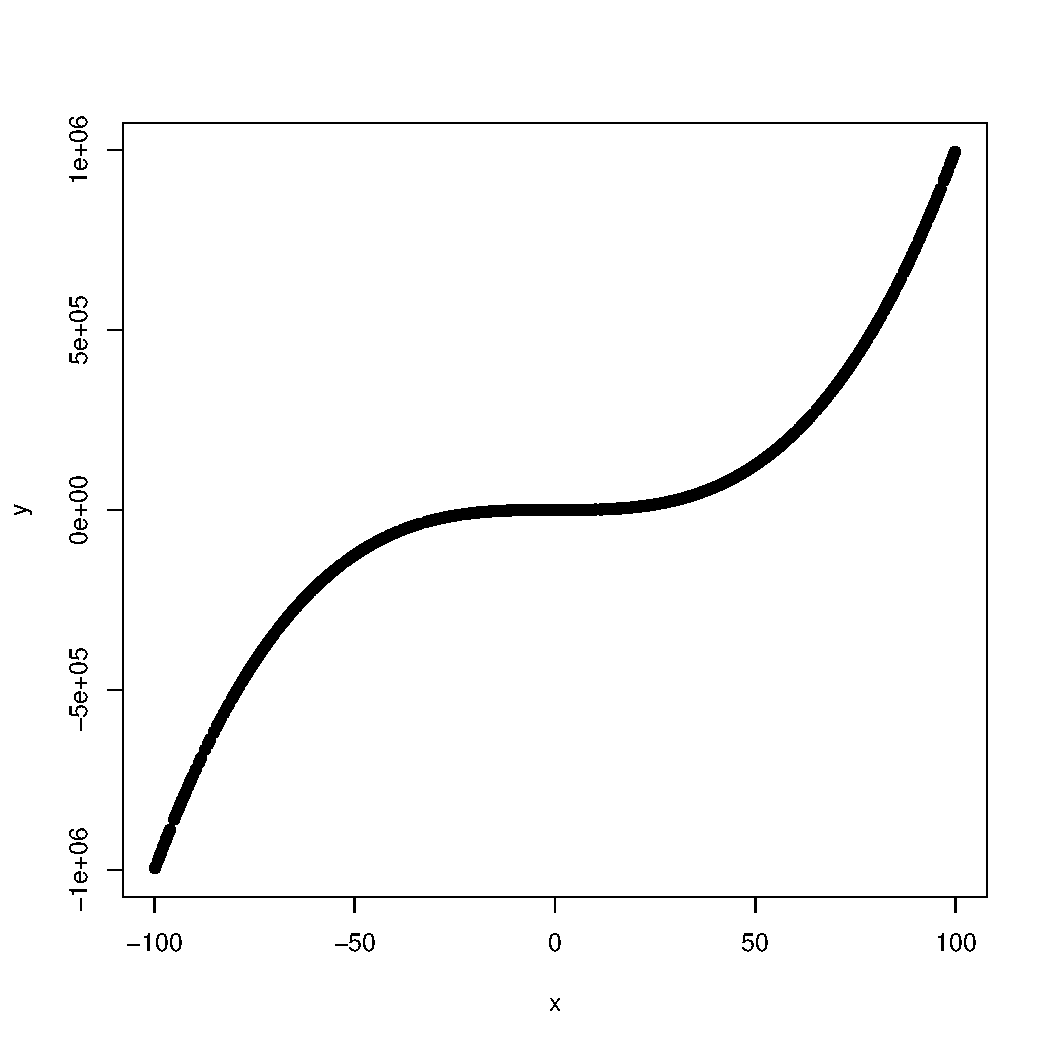
\includegraphics[width=1\textwidth]{xTfunc3.pdf}
    \caption{Función $1 / x$ a partir de mil valores de $X$ desde una distribución uniforme con valores $[-100, 100]$.}
    \label{xTfunc3}
\end{figure}

\begin{figure}
    \begin{subfigure}{.5\textwidth}
        \centering
        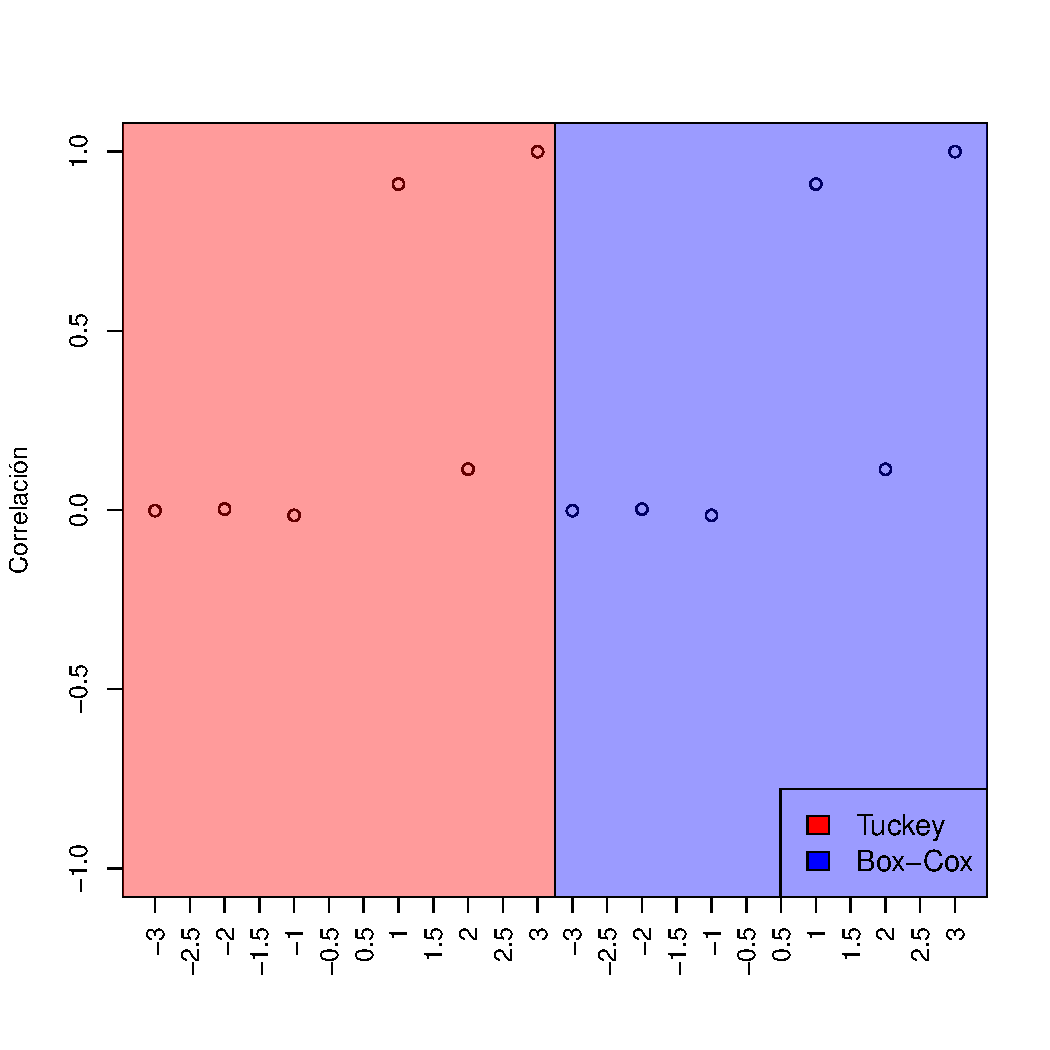
\includegraphics[scale=0.4]{xTcorr3.pdf}
        \caption{$X$ transformada.}
        \label{xTcorr3}
    \end{subfigure}
    \begin{subfigure}{0.5\textwidth}
        \centering
        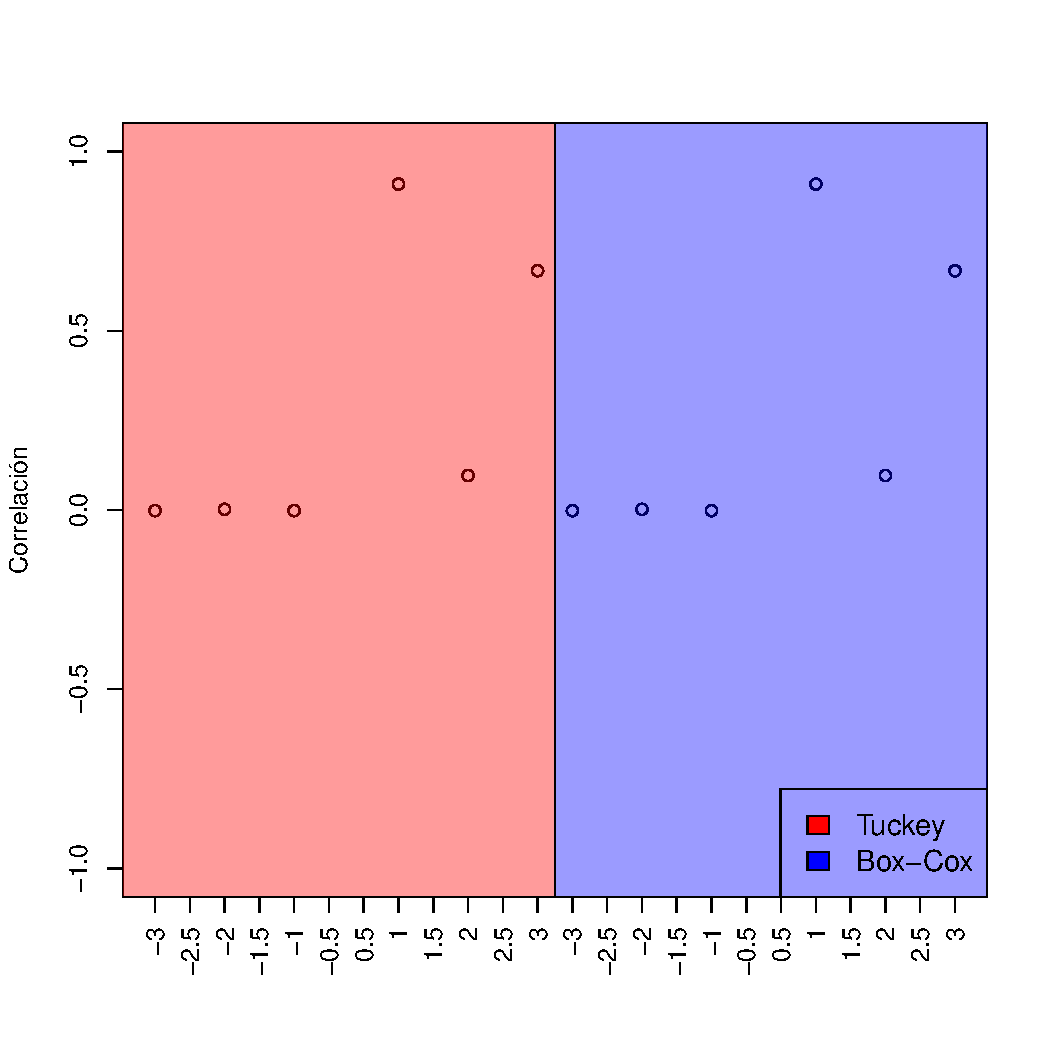
\includegraphics[scale=0.4]{yTcorr3.pdf}
        \caption{$Y$ transformada.}
        \label{yTcorr3}
    \end{subfigure}
    \begin{subfigure}{1\textwidth}
        \centering
        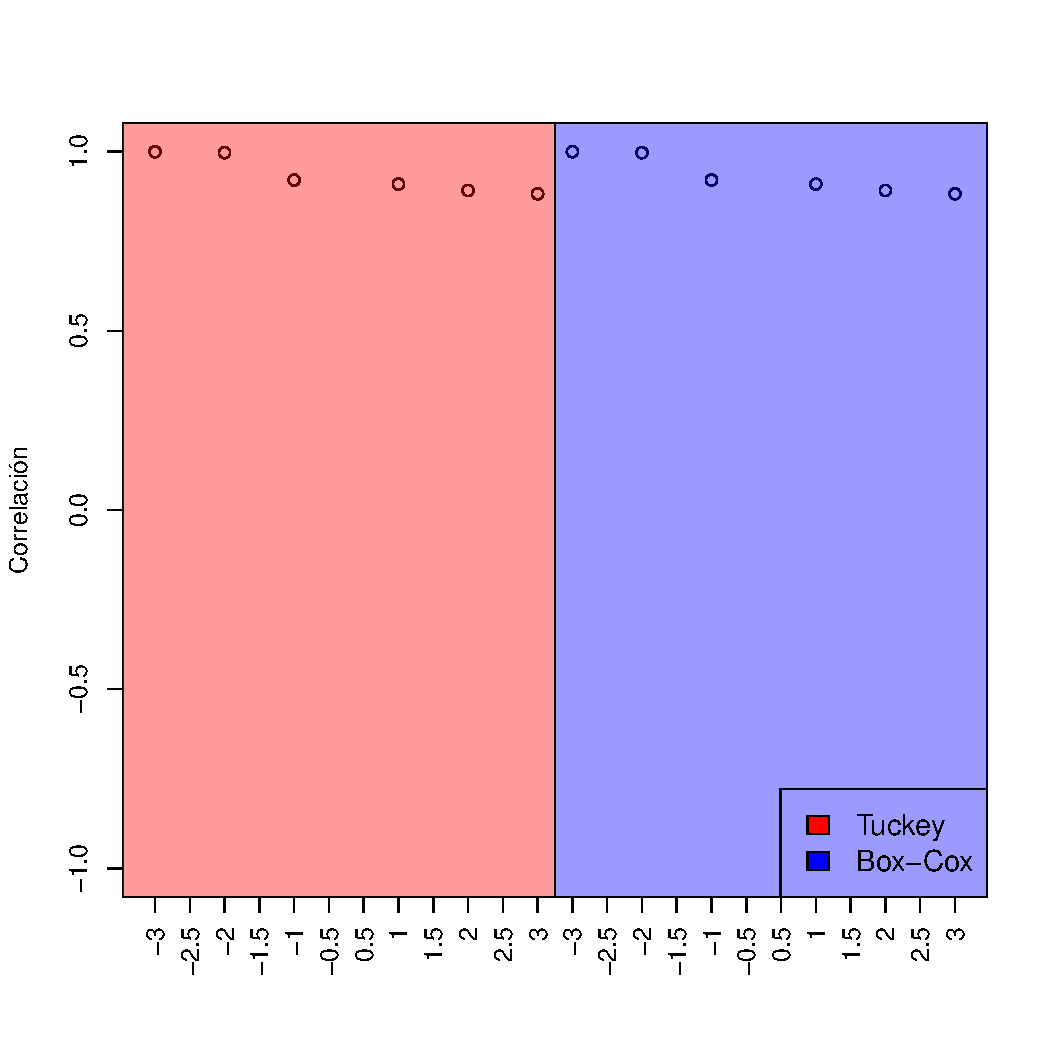
\includegraphics[scale=0.4]{xT_yTcorr3.pdf}
        \caption{$X$ y $Y$ transformadas.}
        \label{yTcorr3}
    \end{subfigure}
    \caption{Gráficas de las correlaciones para la función $1/x$ con transformaciones para $X$, $Y$ y ambas. En el eje horizontal se grafican los valores de $\lambda$, la mitad roja corresponde a transformación de Tuckey, mientras que la azul a la de Box--Cox.}
    \label{corr3}
\end{figure}

\bibliographystyle{plainnat}
\bibliography{Biblio}

\end{document}